\documentclass{beamer}

\mode<presentation>
{
  \usetheme{Warsaw}
  \setbeamercovered{invisible}
}

\setbeamertemplate{navigation symbols}{}

\graphicspath{{./images/}}

\usepackage[english]{babel}
\usepackage{times}
\usepackage[latin1]{inputenc}
\usepackage[T1]{fontenc}
\usepackage{lmodern}
\usepackage{amsmath,amsthm,amssymb}
\usepackage{hyperref}
\usepackage{nccfoots}
\usepackage{subfigure}
\usepackage{outlines}

\renewcommand\thempfootnote{*}

\renewcommand{\t}{$\mathrm{t}$ }
\newcommand{\BHV}{$\mathrm{BHV}$ }
\newcommand{\NP}{$\mathrm{NP}$ }
\newcommand{\MCMC}{$\mathrm{MCMC}$ }
\newcommand{\SPR}{$\mathrm{SPR}$ }

\newcommand{\dts}{\mathrm{2DtT}}
\newcommand{\nni}{\mathrm{NNI}}
\newcommand{\rnni}{\mathrm{rNNI}}
\newcommand{\rnniu}{\mathrm{rNNIu}}
\newcommand{\mdts}{\mathrm{DtT}}
\newcommand{\mdtsu}{\mathrm{DtTu}}
\newcommand{\MH}{\mathrm{MH}}
\newcommand{\ric}{\operatorname{ric}}
\newcommand{\rt}{\mathrm{rt}}
\newcommand{\tp}{\mathrm{tp}}
\newcommand{\W}{\mathcal{W}}
\newcommand{\M}{\mathcal{M}}
\newcommand{\dom}{\mathrm{dom}}

\renewcommand{\O}{\mathcal{O}}

\newtheorem{oobservation}{Trivial observation}

\theoremstyle{example}
\newtheorem{question}{Question}

\setbeamercolor{author}{fg=white}
\setbeamercolor{date}{fg=white}

\title[\url{https://gavruskin.github.io/talks/2016_GSA.pdf}]{The space of sampled ancestor trees\\
@GSA2016}
\author[Alex Gavryushkin \hspace{80pt} These slides:]{\textbf{\large Alex Gavryushkin}}
%\titlegraphic{\includegraphics[height=10mm]{ETH_logo}}
\institute{\includegraphics[height=7.5mm]{ETH_logo_white}}
\date{September 28, 2016}


\begin{document}

{
\usebackgroundtemplate{\includegraphics[height=\paperheight]{ETH_image}}
\begin{frame}[plain]
\setbeamertemplate{footline}{}
\titlepage
\end{frame}
}

\addtocounter{framenumber}{-1}
\addtobeamertemplate{navigation symbols}{}{
	\usebeamerfont{footline}
	\usebeamercolor[fg]{footline}
	\hspace{1em}
	\insertframenumber/\inserttotalframenumber
}

\begin{frame}{Motivation}
\begin{block}

\begin{outline}
\1 General statistics is at least $5$ years ahead of phylostatistics.
\pause
\1 The discrete component of tree space is \emph{the} bottleneck for tree search algorithms.
\pause
\1 What's wrong with trees?
\end{outline}
\end{block}

\pause

\begin{block}{Same as above but with a mortarboard on}
\begin{outline}
\1 \MCMC algorithms
	\2 Improving efficiency $=$ smart proposals
	\2 Point estimates AKA posterior summary
\1 Tree search methods in general
	\2 Semi-convergence
	\2 Valleys
	\2 Terraces
\end{outline}
\end{block}
\end{frame}

\begin{frame}
\begin{block}{Sampled ancestor tree}
\includegraphics[width=\framewidth]{SampledAncestorTree}
\end{block}
\end{frame}

\begin{frame}
\begin{block}{Sampled ancestor tree space}
\includegraphics[width=0.8\framewidth]{SAT}
\end{block}
\end{frame}

\begin{frame}
\begin{block}{The problem}
\includegraphics[width=\framewidth]{SAT_dimension}

\centering
Different dimension
\end{block}
\end{frame}

\begin{frame}{Looks promising}
\begin{block}{G, Whidden, and Matsen. \emph{arXiv,} to appear in July 2016}
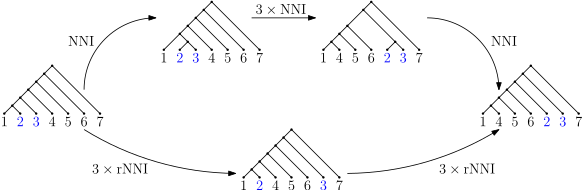
\includegraphics[width = \framewidth]{NNI_VS_rNNI.pdf}
\end{block}

\pause

\begin{block}{And challenging!}
What it the complexity of this graph?
\end{block}

\begin{outline}
\1 Over 25 years to solve for NNI
\1 Over 7 erroneous papers published
\end{outline}

\end{frame}

\begin{frame}{Promising indeed}
\begin{block}{G and Drummond. \emph{JTB,} 2016}
\includegraphics[width=\framewidth]{tauSpace}
\end{block}
\end{frame}

\begin{frame}{More results}
\begin{block}{Mathematical insight}
\begin{outline}
\1 Geometry of discrete time-trees
	\2 Diameter
	\2 Micro- and macro-geometry
\1 Random walking
	\2 Bottle necks
	\2 Curvature
\end{outline}
\end{block}

\pause

\begin{block}{Surprise!}
A better bound for the size of $r$-neighborhoods in $\nni$.
\end{block}
\end{frame}

\begin{frame}{Take home message}

\begin{block}{Our results}
\begin{outline}
\1 Time-trees and classical phylogenetic trees have different geometric and algorithmic properties.
\1 Often, geometric and algorithmic results for classical trees do not scale to time-trees.
\1 Natural and efficient data structures
\end{outline}
\end{block}

\pause

\begin{block}{\small{Future directions}}
\begin{outline}
\1 Applications
	\2 MCMC proposals, local tree rearrangements
	\2 Convergence
	\2 Valleys and terraces
\1 Math/computing:
	\2 Challenging problems that matter
	\2 Connections to other areas of math
	\2 Amenable to various search algorithms
\end{outline}
\end{block}
\end{frame}

\begin{frame}{\href{http://alex.gavruskin.com/pictures/}{\Large{Thank you for your attention!}}}
\thebibliography{9}
\bibliographystyle{alpha}

\scriptsize

\bibitem{Gavruskin2015}
Alex Gavryushkin and Alexei Drummond
\newblock The space of ultrametric phylogenetic trees
\newblock \emph{Journal of Theoretical Biology,} Vol.\,402, 197--208, 2016

\bibitem{chrisErickG2015}
Alex Gavryushkin, Chris Whidden, and Frederick A.\ Matsen IV
\newblock Combinatorics of discrete time-trees: algorithmic insights and open problems
\newblock To appear on the {\em arXiv,} July 2016

\bibitem{GavryushkinGitHub}
\url{https://github.com/gavruskin/tauGeodesic}

\bibitem{GavryushkinGitHub2}
\url{https://github.com/gavruskin/tTauCurvature}
\end{frame}
\end{document}

